\chapter{问题及其解决}
\section{FAQ}
\begin{enumerate}
  \item[Q:]为什么用WINEdt后,汉字显示全部乱码啊?(来自知行论坛)
  \item[A:]先打开WINEdt,然后以utf-8编码打开文件,如下图:\begin{figure}[!ht]\centering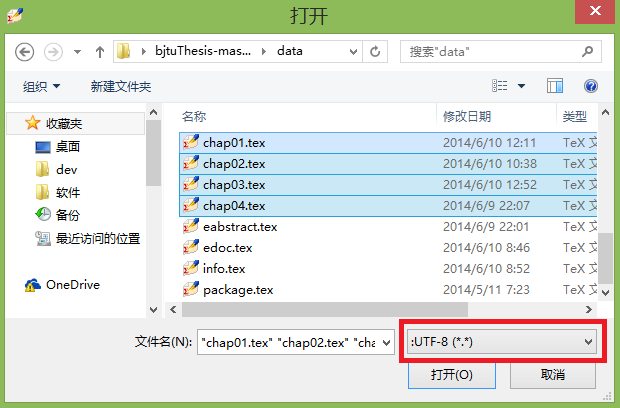
\includegraphics[scale=0.7]{figures/41}\caption{以utf-8编码打开文件}\label{f41}\end{figure}
  \item[Q:]想问一下你的那个模板为啥我打开显示error reading?(来自短信)
  \item[A:]同上个回答。
  \item[Q:]话说用TeXmaker编译好慢阿,用WINEdt也应该如此吧。(来自知行论坛)
  \item[A:]如果系统已安装adobe字体,可以把main.tex的首行改为:\verb|\documentclass[adobefonts,oneside,openany]{bjtuThesis}|,这样编译应该会快一些!
  \item[Q:]我添加了参考文献但点击不跳转;且怎么可以不按引用顺序出现在参考文献页面里,也就是说我先引用的文献标号为1,但我不希望它排在第一位;(来自邮件)
  \item[A:]谁帮我回答一下。
  \item[Q:]还有就是我附录中文翻译里面的section怎么不显示在目录里?(来自短信)
  \item[A:]用\verb|\section*{}|。
  \item[Q:]引用文献怎么是绿色的?能改为黑色么?还有目录的红色我也想知道怎么改为黑色...(来自短信)
  \item[A:]引用文献、目录有颜色是因为它们是链接,默认为绿、红。最新的模板已支持自定义链接颜色,具体地,见main.tex里的注释。
\end{enumerate}
\section{反馈意见和建议}
关于本模板的意见和建议可发送邮件至\href{mailto:10271061@bjtu.edu.cn}{10271061@bjtu.edu.cn}.
